\documentclass[a4paper]{article}
\usepackage{amsmath, amssymb, bm}
\usepackage[margin=1in]{geometry}
\usepackage[table,xcdraw]{xcolor}
\usepackage{graphicx}
\usepackage{subfigure}
\begin{document}
\begin{titlepage}
  \centering
    {\huge \bf Assignment 3\par}
    \vspace{1cm}
    {\Large Computational Intelligence, SS2018\par}
    \vspace{1cm}
    \begin{tabular}{|l|l|l|}
      \hline
      \multicolumn{3}{|c|}{\textbf{Team Members}}   \\ \hline
      Last name & First name & Matriculation Number \\ \hline
      Lee       & Eunseo     & 11739623             \\ \hline
      Shadley   & Alex       & 11739595             \\ \hline
      Lee       & Dayeong    & 11730321             \\ \hline
    \end{tabular}
\end{titlepage}

\section{Linear SVM}
\section{Nonlinear (kernal) SVM}

\subsection*{Results}

\noindent
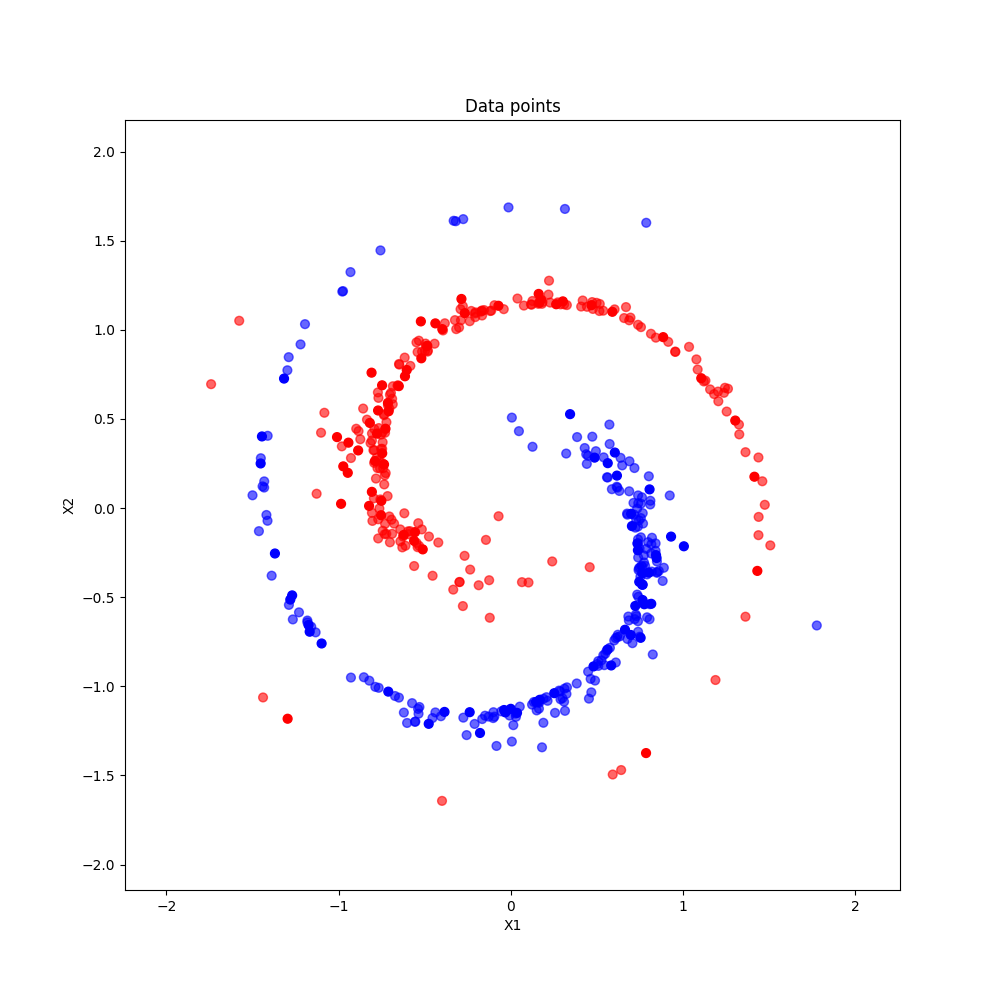
\includegraphics[width=0.5\textwidth]{nonlinear_data.png}%
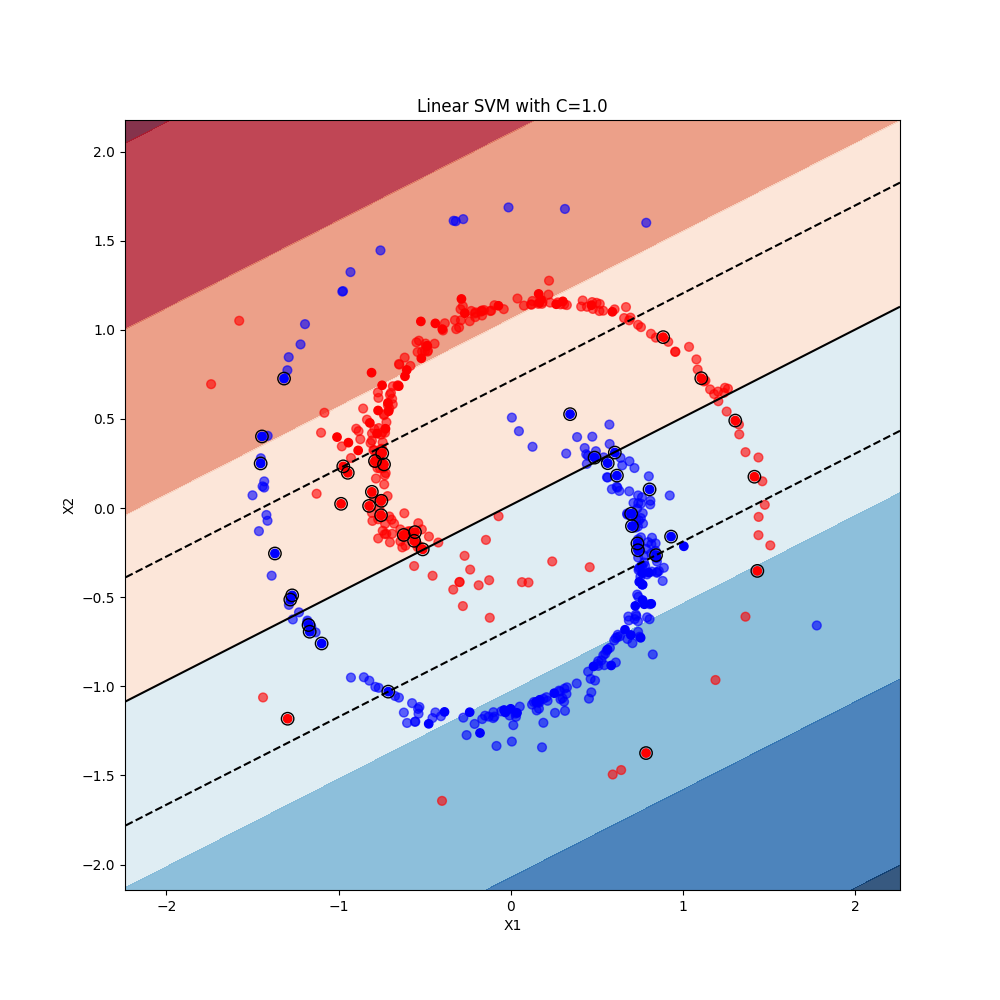
\includegraphics[width=0.5\textwidth]{linear_fit.png}\\[2em]
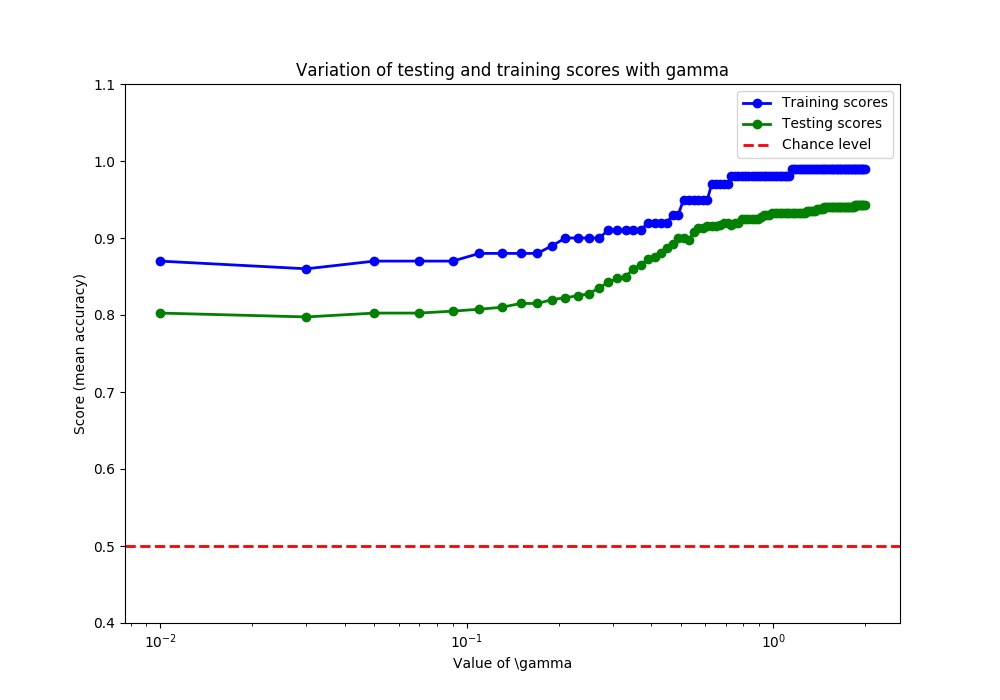
\includegraphics[width=0.5\textwidth]{rbf_error.png}%
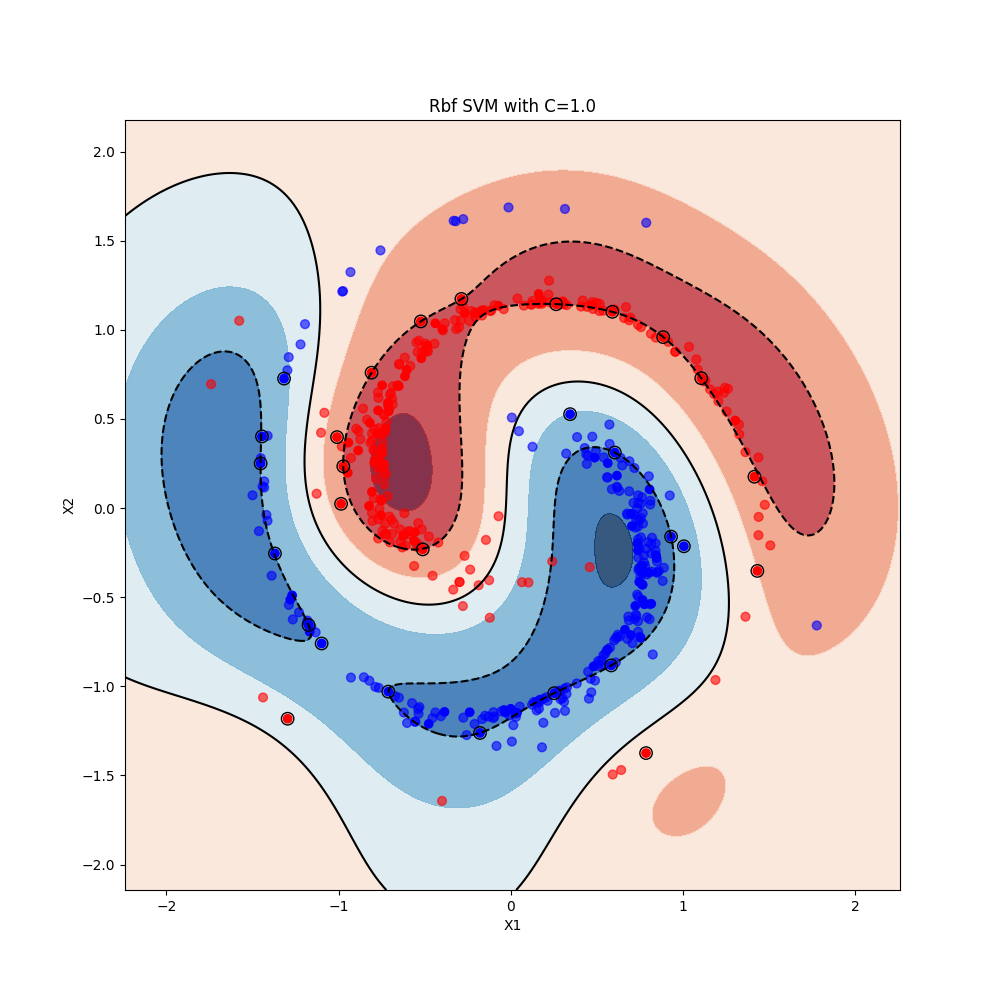
\includegraphics[width=0.5\textwidth]{rbf_fit.png}\\[2em]
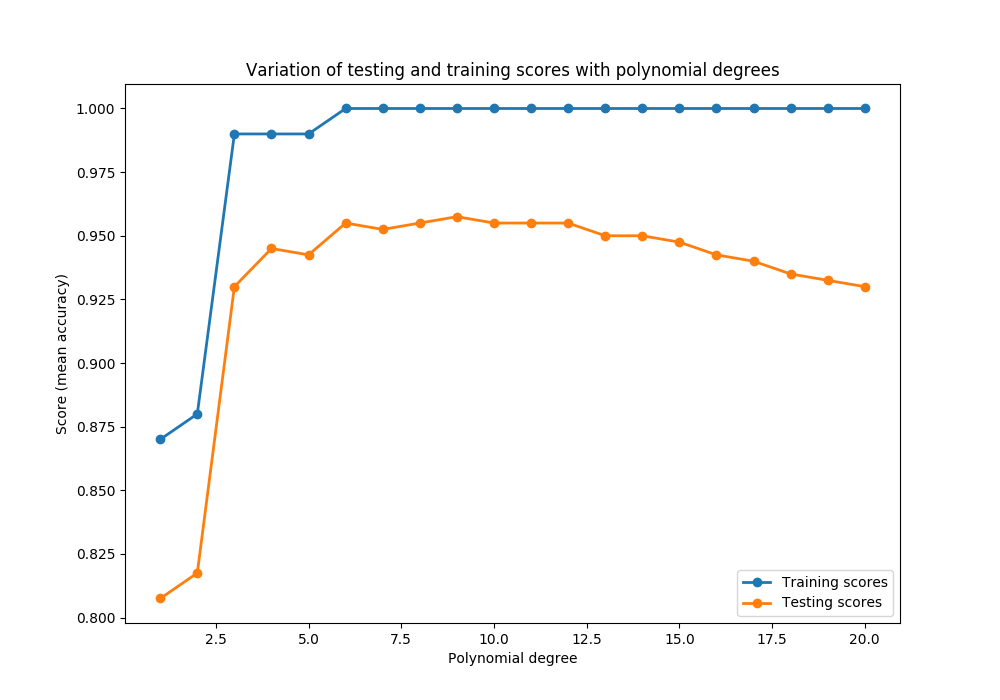
\includegraphics[width=0.5\textwidth]{poly_error.png}%
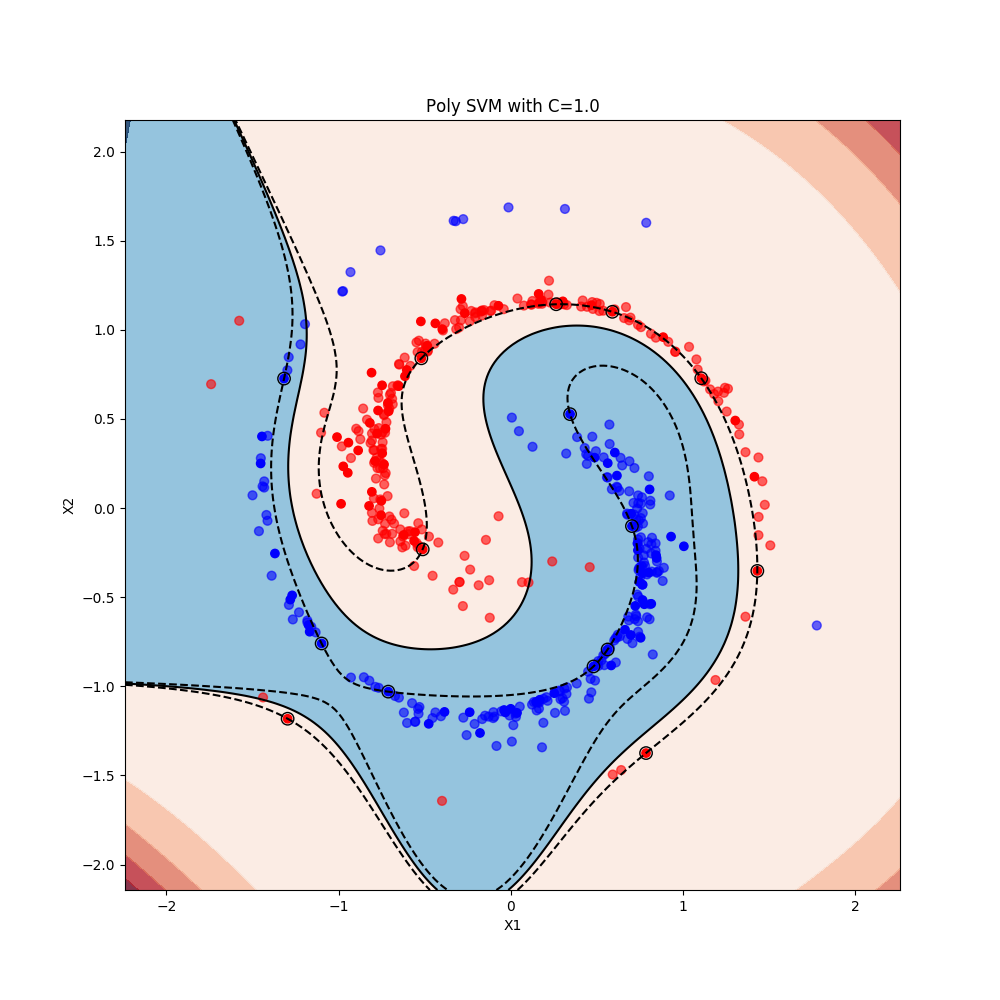
\includegraphics[width=0.5\textwidth]{poly_fit.png}\par

The above figures depict (left to right, top to bottom)

\begin{enumerate}
	\item Training data used for all algorithms
	\item A Linear SVM convergence
	\item Error in a RBF SVM plotted against the gamma value used in the kernel
	\item The most proficient RBF SVM
	\item Error in a Polynomial SVM plotted against the polynomial degree used in the kernel
	\item The most proficient Polynomial SVM
\end{enumerate}


\subsection*{Discussion}

Our Polynomial SVM had the best performance with a score of .9575 with degree 9.  The RBF SVM performed second best, scoring .9425 with a gamma of 1.85, and the Linear SVM exhibited the worst performance at .8125 .  Since the data is not linearly seperable, it is clear why the Linear SVM performed poorly.  The polynomial model outperformed the RBF model because it was able to more accurately model the central region $(-.5 < x_1, x_2 < .5)$.  It is worth noting that both models struggled with this region, with both having a significant number of misclassified examples in the region.

In general, it can be seen that a high number of Support Vectors correlates to complex decision boundaries, although this is obviously not the case for linear models.  Despite the testing results, I believe the RBF model produces a better generalization of the data, as it places the decision boundary more accurately between data points than other models.

\section{Multiclass classification}
\end{document}
